% This is the Reed College LaTeX thesis template. Most of the work
% for the document class was done by Sam Noble (SN), as well as this
% template. Later comments etc. by Ben Salzberg (BTS). Additional
% restructuring and APA support by Jess Youngberg (JY).
% Your comments and suggestions are more than welcome; please email
% them to cus@reed.edu
%
% See https://www.reed.edu/cis/help/LaTeX/index.html for help. There are a
% great bunch of help pages there, with notes on
% getting started, bibtex, etc. Go there and read it if you're not
% already familiar with LaTeX.
%
% Any line that starts with a percent symbol is a comment.
% They won't show up in the document, and are useful for notes
% to yourself and explaining commands.
% Commenting also removes a line from the document;
% very handy for troubleshooting problems. -BTS

% As far as I know, this follows the requirements laid out in
% the 2002-2003 Senior Handbook. Ask a librarian to check the
% document before binding. -SN

%%
%% Preamble
%%
% \documentclass{<something>} must begin each LaTeX document
\documentclass[12pt,oneside]{reedthesis}
% Packages are extensions to the basic LaTeX functions. Whatever you
% want to typeset, there is probably a package out there for it.
% Chemistry (chemtex), screenplays, you name it.
% Check out CTAN to see: https://www.ctan.org/
%%
\usepackage{graphicx,latexsym}
\usepackage{amsmath}
\usepackage{amssymb,amsthm}
\usepackage{longtable,booktabs,setspace}
\usepackage{chemarr} %% Useful for one reaction arrow, useless if you're not a chem major
\usepackage[hyphens]{url}
% Added by CII
\usepackage[hidelinks]{hyperref}
\usepackage{lmodern}
\usepackage{float}
\floatplacement{figure}{H}
% Thanks, @Xyv
\usepackage{calc}
% End of CII addition
\usepackage{rotating}

% Next line commented out by CII
%%% \usepackage{natbib}
% Comment out the natbib line above and uncomment the following two lines to use the new
% biblatex-chicago style, for Chicago A. Also make some changes at the end where the
% bibliography is included.
%\usepackage{biblatex-chicago}
%\bibliography{thesis}
% \ifxetex
%   \usepackage{polyglossia}
%   \setmainlanguage{spanish}
%   % Tabla en lugar de cuadro
%   \gappto\captionsspanish{\renewcommand{\tablename}{Tabla}
%           \renewcommand{\listtablename}{Índice de tablas}}
% \else
%   \usepackage[spanish,es-tabla]{babel}
% \fi

% Added by CII (Thanks, Hadley!)
% Use ref for internal links
\renewcommand{\hyperref}[2][???]{\autoref{#1}}
\def\chapterautorefname{chapter}
\def\sectionautorefname{section}
\def\subsectionautorefname{subsection}
% End of CII addition

% Added by CII
\usepackage{caption}
\captionsetup{width=5in}
% End of CII addition

% \usepackage{times} % other fonts are available like times, bookman, charter, palatino

% Syntax highlighting #22

% To pass between YAML and LaTeX the dollar signs are added by CII
\title{Ondas de Rossby planetarias en la circulación atmosférica del hemisferio sur y su influencia en Sudamérica}
\author{Lic. Elio Campitelli}
% The month and year that you submit your FINAL draft TO THE LIBRARY (May or December)
\date{BUENOS AIRES, 2023}
\division{Facultad de Ciencias Exactas y Naturales}
\advisor{Carolina Vera}
\institution{Universidad de Buenos Aires}
\degree{Tesis presentada para optar al título de Doctore de la Universidad de Buenos Aires en el Área de Ciencias de la Atmósfera y los Océanos}
%If you have two advisors for some reason, you can use the following
% Uncommented out by CII
\altadvisor{Leandro Diaz}
\consejere{Claudio Menendez}
\place{Centro de Investigaciones del Mar y la Atmósfera. CONICET-UBA}
% End of CII addition

%%% Remember to use the correct department!
\department{Departamento de Ciencias de la Atmósfera y los Océanos}
% if you're writing a thesis in an interdisciplinary major,
% uncomment the line below and change the text as appropriate.
% check the Senior Handbook if unsure.
%\thedivisionof{The Established Interdisciplinary Committee for}
% if you want the approval page to say "Approved for the Committee",
% uncomment the next line
%\approvedforthe{Committee}

% Added by CII
%%% Copied from knitr
%% maxwidth is the original width if it's less than linewidth
%% otherwise use linewidth (to make sure the graphics do not exceed the margin)
\makeatletter
\def\maxwidth{ %
  \ifdim\Gin@nat@width>\linewidth
    \linewidth
  \else
    \Gin@nat@width
  \fi
}
\makeatother

\makeatletter
\renewcommand{\@chapapp}{Capítulo}
\makeatother

% From {rticles}
\newlength{\csllabelwidth}
\setlength{\csllabelwidth}{3em}
\newlength{\cslhangindent}
\setlength{\cslhangindent}{1.5em}
% for Pandoc 2.8 to 2.10.1
\newenvironment{cslreferences}%
  {}%
  {\par}
% For Pandoc 2.11+
% As noted by @mirh [2] is needed instead of [3] for 2.12
\newenvironment{CSLReferences}[2] % #1 hanging-ident, #2 entry spacing
 {% don't indent paragraphs
  \setlength{\parindent}{0pt}
  % turn on hanging indent if param 1 is 1
  \ifodd #1 \everypar{\setlength{\hangindent}{\cslhangindent}}\ignorespaces\fi
  % set entry spacing
  \ifnum #2 > 0
  \setlength{\parskip}{#2\baselineskip}
  \fi
 }%
 {}
\usepackage{calc} % for calculating minipage widths
\newcommand{\CSLBlock}[1]{#1\hfill\break}
\newcommand{\CSLLeftMargin}[1]{\parbox[t]{\csllabelwidth}{#1}}
\newcommand{\CSLRightInline}[1]{\parbox[t]{\linewidth - \csllabelwidth}{#1}}
\newcommand{\CSLIndent}[1]{\hspace{\cslhangindent}#1}

\renewcommand{\contentsname}{Índice}
% End of CII addition

\setlength{\parskip}{0pt}

% Added by CII

\providecommand{\tightlist}{%
  \setlength{\itemsep}{0pt}\setlength{\parskip}{0pt}}

\Acknowledgements{
I want to thank a few people.
}

\Dedication{
You can have a dedication here if you wish.
}

\Preface{

}

\Abstract{
asbal albal

fdsg dfg sdfg
}


\Resumen{
Este trabajo tiene como objetivo avanzar en la caracterización y entendimiento de la circulación zonalmente asimétrica del Hemisferio Sur en escalas estacionales y más largas.
Para esto se analizaron datos de reanálisis de ERA5 y corridas históricas de CMIP6.
Se computaron las Funciones Empíricas Ortogonales Complejas (cEOF, por sus siglas en inglés) de las anomalías zonales de altura geopotencial en 200 hPa y 50 hPa.
Éstas son similares a las EOF tradicionales pero permiten caracterizar patrones de variabilidad que tienen fase además de amplitud.

El cEOF1 representa la variabilidad de la onda zonal 1 en la estratosfera y está estrechamente con las anomalías en el ozono.
El cEOF2, por su parte, representa un patrón de onda 3 con magnitud máxima en el sector del Pacífico, que resulta ser una descripción alternativa de los modos PSA.
El análisis de este modo indica que se trata de un modo de variabilidad interna de la atmósfera subtropical que toma una fase preferencial en respuesta al forzante tropical.
Sólo el cEOF2 está asociado a impactos en la superficie.

Para estudiar la relación entre estos modos de variabilidad en la circulación asimétrica y el Modo Anular del Sur (SAM), que representa principalmente variabilidad simétrica, separamos la variabilidad del SAM en su parte zonalmente simétrica (S-SAM) y asimétrica (A-SAM).
En base a la separación del SAM en S-SAM y A-SAM, observamos que la fase de 90º del cEOF2 tiene una correlación extremadamente alta con el A-SAM, sugiriendo que se trata de dos metodologías que observan el mismo fenómeno o que la parte asimétrica del SAM sea en realidad una contaminación estadística del modo PSA en un SAM más zonalmente simétrico.

Finalmente, analizamos estos modos de variabilidad en las corridas históricas del CMIP6.
Encontramos que la representación de los modos es muy variable entre modelos e incluso entre los miembros de un mismo modelo, sin embargo, la media multimodelo representa los modos muy bien.
Sin embargo, la mayoría de los modelos exageran la relación entre los modos y la temperatura de la superficie del mar
}

	\usepackage{setspace}\onehalfspacing
\usepackage[spanish]{babel}
	\usepackage{booktabs}
\usepackage{longtable}
\usepackage{array}
\usepackage{multirow}
\usepackage{wrapfig}
\usepackage{float}
\usepackage{colortbl}
\usepackage{pdflscape}
\usepackage{tabu}
\usepackage{threeparttable}
\usepackage{threeparttablex}
\usepackage[normalem]{ulem}
\usepackage{makecell}
\usepackage{xcolor}
% End of CII addition
%%
%% End Preamble
%%
%
\begin{document}

% Everything below added by CII
  \maketitle

\frontmatter % this stuff will be roman-numbered
\pagestyle{empty} % this removes page numbers from the frontmatter

  \begin{resumen}
    Este trabajo tiene como objetivo avanzar en la caracterización y entendimiento de la circulación zonalmente asimétrica del Hemisferio Sur en escalas estacionales y más largas.
    Para esto se analizaron datos de reanálisis de ERA5 y corridas históricas de CMIP6.
    Se computaron las Funciones Empíricas Ortogonales Complejas (cEOF, por sus siglas en inglés) de las anomalías zonales de altura geopotencial en 200 hPa y 50 hPa.
    Éstas son similares a las EOF tradicionales pero permiten caracterizar patrones de variabilidad que tienen fase además de amplitud.

    El cEOF1 representa la variabilidad de la onda zonal 1 en la estratosfera y está estrechamente con las anomalías en el ozono.
    El cEOF2, por su parte, representa un patrón de onda 3 con magnitud máxima en el sector del Pacífico, que resulta ser una descripción alternativa de los modos PSA.
    El análisis de este modo indica que se trata de un modo de variabilidad interna de la atmósfera subtropical que toma una fase preferencial en respuesta al forzante tropical.
    Sólo el cEOF2 está asociado a impactos en la superficie.

    Para estudiar la relación entre estos modos de variabilidad en la circulación asimétrica y el Modo Anular del Sur (SAM), que representa principalmente variabilidad simétrica, separamos la variabilidad del SAM en su parte zonalmente simétrica (S-SAM) y asimétrica (A-SAM).
    En base a la separación del SAM en S-SAM y A-SAM, observamos que la fase de 90º del cEOF2 tiene una correlación extremadamente alta con el A-SAM, sugiriendo que se trata de dos metodologías que observan el mismo fenómeno o que la parte asimétrica del SAM sea en realidad una contaminación estadística del modo PSA en un SAM más zonalmente simétrico.

    Finalmente, analizamos estos modos de variabilidad en las corridas históricas del CMIP6.
    Encontramos que la representación de los modos es muy variable entre modelos e incluso entre los miembros de un mismo modelo, sin embargo, la media multimodelo representa los modos muy bien.
    Sin embargo, la mayoría de los modelos exageran la relación entre los modos y la temperatura de la superficie del mar
  \end{resumen}
  \begin{abstract}
    asbal albal

    fdsg dfg sdfg
  \end{abstract}

  \begin{acknowledgements}
    I want to thank a few people.
  \end{acknowledgements}

  \hypersetup{linkcolor=black}
  \setcounter{secnumdepth}{2}
  \setcounter{tocdepth}{2}
  \tableofcontents

  \listoftables

  \listoffigures
  \begin{dedication}
    You can have a dedication here if you wish.
  \end{dedication}
\mainmatter % here the regular arabic numbering starts
\pagestyle{fancyplain} % turns page numbering back on

\hypertarget{introducciuxf3n}{%
\chapter{Introducción}\label{introducciuxf3n}}

Explicar onda 3 y demás. Resumir resultados de la tesis de licenciatura.
Explicar motivación para huirle a Fourier.

Acá irían figuras mostrando los problemas con la onda3 de fourier (que están \href{http://htmlpreview.github.io/?https://github.com/eliocamp/onda3/blob/master/30-no-zw.html}{acá}).
\begin{enumerate}
\def\labelenumi{\arabic{enumi}.}
\tightlist
\item
  Los puntos donde se dan los máximos de la onda 3 no son covariantes.
\item
  Los patrones de correlación asociados a cada punto no muetran una onda 3
\item
  Tanto wavelets como el análisis de ``covarianza por gajos'' muestran una modulación de la amplitud importante.
\end{enumerate}
\hypertarget{visiuxf3n-tradicional-dela-onda-3-del-hemisferio-sur}{%
\section{Visión tradicional dela onda 3 del hemisferio sur}\label{visiuxf3n-tradicional-dela-onda-3-del-hemisferio-sur}}

\hypertarget{problemas}{%
\subsection{Problemas}\label{problemas}}

\hypertarget{modos-de-variabilidad-de-la-circulaciuxf3n-zonalmente-asimuxe9trica}{%
\chapter{Modos de variabilidad de la circulación zonalmente asimétrica}\label{modos-de-variabilidad-de-la-circulaciuxf3n-zonalmente-asimuxe9trica}}

Acá iría básicamente \href{https://github.com/eliocamp/shceof}{el paper de cEOF}.

\hypertarget{datos-y-muxe9todos}{%
\section{Datos y métodos}\label{datos-y-muxe9todos}}

\hypertarget{funciones-ortogonales-complejas-ceof}{%
\subsection{Funciones ortogonales complejas (cEOF)}\label{funciones-ortogonales-complejas-ceof}}


\begin{figure}
\centering
\includegraphics{thesis_files/figure-latex/eof-naive-1.pdf}
\caption{\label{fig:eof-naive}Spatial patterns of the four leading EOFs of SON geopotential height zonal anomalies at 50 hPa south of 20º S for the 1979 -- 2019 period (arbitrary units).}
\end{figure}
En el análisis EOF estándar, las ondas zonales pueden aparecer como pares de EOFs (posiblemente degenerados) que representan patrones similares pero desplazados en fase (\textbf{horel1984?}).
La figura \ref{fig:eof-naive} muestra los cuatro EOFs principales de las anomalías zonales de altura geopotencial SON a 50 hPa al sur de 20º S.
Está claro que los dos primeros EOFs representan un único patrón de onda zonal 1 con variación de fase y los dos últimos representan un patrón con variación de fase similar con un número de onda más alto y tres centros de acción desplazados 1/4 de longitud de onda (90º en el espacio de frecuencias).

Para describir la naturaleza variable en fase de estos dos patrones de onda, una forma es combinar cada par de EOF en índices de amplitud y fase.
Así, por ejemplo, la amplitud de la onda 1-como EOF podría medirse como \(\sqrt{\mathrm{PC1}^2 + \mathrm{PC2}^2}\) y su fase como \(\tan^{-1} \left ( \frac{\mathrm{PC2}}{\mathrm{PC1}} \right )\) (donde \(\mathrm{PC1}\) y \(\mathrm{PC2}\) son las series temporales asociadas a cada EOF).
Sin embargo, esto se basa en la inspección visual de los patrones espaciales y sólo funciona correctamente si ambas fases aparecen claramente en diferentes EOFs, lo que no está garantizado por construcción.
En particular, esto no funciona con el patrón de la onda 1 representado como el EOF principal en las anomalías zonales de altura geopotencial de 200 hPa (no mostrado).

Por otro lado, una alternativa mejor para describir ondas con variación de fase es utilizar el análisis de Funciones Ortogonales Empíricas Complejas (cEOF) (\textbf{horel1984?}).
Cada cEOF es un conjunto de patrones espaciales de valor complejo y series temporales.
Los componentes real e imaginario del patrón espacial complejo pueden considerarse como la representación de dos patrones espaciales que están desplazados 1/4 de longitud de onda por construcción, de forma similar a EOF1 y EOF2 en la Figura \ref{fig:eof-naive}.
En este documento utilizamos los términos 0º cEOF y 90º cEOF para referirnos a cada parte del cEOF completo.
El campo real reconstruido por cada cEOF es entonces la combinación lineal de los dos campos espaciales ponderados por sus respectivas series temporales.
Esto es análogo a cómo cualquier onda sinusoidal puede construirse mediante la suma de una onda sinusoidal y una onda cosenoidal con diferente amplitud pero fase constante.
Esto significa que los CEOF representan de forma natural patrones ondulatorios de fase variable que cambian tanto de ubicación como de amplitud.

Por ejemplo, cuando la fase de la onda coincide con la fase 0º, entonces la serie temporal de fase 0º es positiva y la serie temporal de fase 90º es cero.
Del mismo modo, cuando la fase de la onda coincide con la fase 90º, la serie temporal de fase 90º es positiva y la serie temporal de fase 0º es cero.
Las fases intermedias tienen valores distintos de cero en ambas series temporales.

Los EOF tradicionales no son únicos, sino que se definen hasta el signo, que corresponde a una rotación en el plano complejo de 0 o \(\pi\).
Del mismo modo, los cEOF se definen hasta una rotación en el plano complejo de cualquier valor entre 0 y \(2\pi\) (\textbf{horel1984?}).

Los cEOF se calculan de la misma forma que los EOF tradicionales, salvo que primero se aumentan los datos calculando su señal analítica.
Se trata de un número complejo cuya parte real es la serie original y cuya parte imaginaria son los datos originales desplazados 90º en cada frecuencia espectral, es decir, su transformada de Hilbert.
La transformada de Hilbert suele entenderse en términos de señal variable en el tiempo.
Sin embargo, en este trabajo aplicamos la transformada de Hilbert en cada círculo de latitud y en cada momento considerado (es decir, la señal sólo depende de la longitud).
Dado que cada círculo de latitud es un dominio periódico, este procedimiento no sufre efectos de borde.

Primero aplicamos el análisis cEOF a las anomalías zonales de altura geopotencial al sur de 20ºS a 50 y a 200 hPa.
La figura \ref{fig:ceofs-1} a.1 muestra los patrones espaciales de los dos cEOF principales.
La fase de 0º se representa con contornos sombreados y la fase de 90º, con contornos negros.
Las dos fases del cEOF líder son muy similares a los dos EOF líderes mostrados en la Figura \ref{fig:eof-naive} y representan un patrón de onda zonal 1; la fase de 0º es aproximadamente el EOF1 y la fase de 90º es aproximadamente el EOF2).


\begin{table}

\caption{\label{tab:corr-ceof-splitted}Coefficient of determination (\(r^2\)) between the time series of the absolute magnitude of complex EOFs computed separately at 200 hPa and 50 hPa (p-values lower than 0.01 in bold).}
\centering
\begin{tabular}[t]{l>{}r>{}r>{}r}
\toprule
\multicolumn{1}{c}{} & \multicolumn{3}{c}{50 hPa} \\
\cmidrule(l{3pt}r{3pt}){2-4}
200 hPa & cEOF1 & cEOF2 & cEOF3\\
\midrule
cEOF1 & \textbf{0.29} & 0.01 & 0.03\\
cEOF2 & 0.00 & \textbf{0.59} & 0.02\\
cEOF3 & 0.00 & 0.00 & 0.01\\
\bottomrule
\end{tabular}
\end{table}
La tabla \ref{tab:corr-ceof-splitted} muestra el coeficiente de determinación entre las series temporales de la amplitud de cada cEOF a través de los niveles.
Existe un alto grado de correlación entre la magnitud de los respectivos cEOF1 y cEOF2 en cada nivel.
Los patrones espaciales de los cEOF de 50 hPa y 200 hPa también son similares (no se muestra).

Tanto la similitud del patrón espacial como la alta correlación temporal de los cEOF calculados a 50 hPa y 200 hPa sugieren que se trata, en gran medida, de modos de variabilidad conjunta.
Esto motiva la decisión de realizar los cEOF conjuntamente entre niveles.
Por lo tanto, los cEOF se calcularon utilizando datos de ambos niveles al mismo tiempo.
En ese sentido, cada cEOF tiene un componente espacial que depende de la longitud, la latitud y el nivel, y un componente temporal que depende sólo del tiempo.

Como ya se ha dicho, la elección de las fases es arbitraria e igualmente válida.
Pero para facilitar la interpretación, elegimos la fase de cada cEOF de modo que o bien el cEOF de 0º o bien el cEOF de 90º estén alineados con variables significativas en nuestro análisis.
Este procedimiento no crea correlaciones espurias, sólo toma una relación existente y la alinea con una fase específica.

El análisis preliminar mostró que el primer cEOF estaba estrechamente relacionado con la onda zonal 1 del COT y el segundo cEOF estaba estrechamente relacionado con el ENSO.
Por lo tanto, elegimos la fase del cEOF1 de forma que la serie temporal correspondiente al cEOF1 de 0º tuviera la máxima correlación con la onda zonal 1 del COT entre 75°S and 45°S.
Del mismo modo, elegimos la fase del cEOF2 de modo que el coeficiente de determinación entre el ONI y el cEOF2 de 0º sea mínimo, lo que también casi maximiza la correlación con el cEOF2 de 90º.

En la sección @ref(precipitación) mostramos regresiones de precipitación y temperatura asociadas a fases intermedias.
Para esos gráficos, rotamos los cEOFs en 1/4 de longitud de onda multiplicando las series temporales complejas por \(\cos(\pi/4) + i\sin(\pi/4)\) y calculando la regresión sobre esas series temporales rotadas.

Aunque calculamos estas componentes principales complejas utilizando datos de 1979 a 2019, extendimos las series temporales complejas hasta el periodo 1950 - 1978 proyectando las anomalías zonales mensuales de altura geopotencial normalizadas por nivel al sur de 20ºS sobre los patrones espaciales correspondientes.

Realizamos regresiones lineales para cuantificar la asociación entre los cEOF y otras variables (por ejemplo, altura geopotencial, temperatura, precipitaciones y otras).
Para cada cEOF, calculamos mapas de regresión ajustando un modelo lineal múltiple que incluía tanto la fase de 0º como la de 90º.
Para obtener los coeficientes lineales de una variable \(X\) con la fase 0º y 90º de cada cEOF ajustamos la ecuación

\[
X(\lambda, \phi, t) = \alpha(\lambda, \phi) \operatorname{cEOF_{0º}} + \beta(\lambda, \phi) \operatorname{cEOF_{90º}} + X_0(\lambda, \phi) + \epsilon(\lambda, \phi, t)
\]

donde \(\lambda\) y \(\phi\) son la longitud y la latitud, \(t\) es el tiempo, \(\alpha\) y \(\beta\) son los coeficientes de regresión lineal para las fases de 0º y 90º respectivamente, \(X_0\) y \(\epsilon\) son la constante y los términos de error respectivamente.

Evaluamos la significancia estadística mediante una prueba t de dos caras y, en el caso de los mapas de regresión, los valores p se ajustaron controlando la Tasa de Falsos Descubrimientos (\textbf{benjamini1995?}; \textbf{wilks2016?}) para evitar resultados engañosos derivados del elevado número de regresiones (\textbf{walker1914?}; \textbf{katz1991?}).

\hypertarget{primavera}{%
\section{Primavera}\label{primavera}}

\hypertarget{descripciuxf3n-de-los-modos}{%
\subsection{Descripción de los modos}\label{descripciuxf3n-de-los-modos}}

\hypertarget{espaciales}{%
\subsubsection{Patrones espaciales}\label{espaciales}}


\begin{figure}
\centering
\includegraphics{thesis_files/figure-latex/ceofs-1-1.pdf}
\caption{\label{fig:ceofs-1}Spatial patterns for the two leading cEOFs of SON geopotential height zonal anomalies at 50 hPa and 200 hPa for the 1979 -- 2019 period. The shading (contours) corresponds to 0º (90º) phase. Arbitrary units. The proportion of variance explained for each mode with respect to the zonal mean is indicated in parenthesis.}
\end{figure}

\begin{figure*}
\includegraphics{thesis_files/figure-latex/extended-series-1} \caption{Time series of the two leading cEOFs of SON geopotential height zonal anomalies at 50 hPa and 200 hPa. cEOF1 (row a) and cEOF2 (row b) separated in their 0º (column 1) and 90º (column 2) phase. Dark straight line is the linear trend. Black horizontal and vertical line mark the mean value and range of each time series, respectively.}\label{fig:extended-series}
\end{figure*}
Para describir la variabilidad de las anomalías zonales de la circulación, en las Figuras \ref{fig:ceofs-1} y \ref{fig:extended-series} se muestran las partes espacial y temporal de los dos primeros modos cEOF de las anomalías zonales de la altura geopotencial a 50 hPa y 200 hPa, calculados conjuntamente en ambos niveles.
El primer modo (cEOF1) explica el 82\% de la varianza de los campos anómalos zonalmente, mientras que el segundo modo (cEOF2) explica una fracción menor (7\%).
En los patrones espaciales (Fig. \ref{fig:ceofs-1}), las fases de 0º y 90º están en cuadratura por construcción, de modo que cada cEOF describe un único patrón ondulatorio cuya amplitud y posición (es decir, fase) está controlada por la magnitud y fase del cEOF temporal.
Los patrones de onda descritos por estos cEOF coinciden con los patrones observados en los EOF estándar de la Figura \ref{fig:eof-naive}.

El cEOF1 (Fig. \ref{fig:ceofs-1} columna 1) es un patrón de onda hemisférica 1 con amplitud máxima en latitudes altas.
A 50 hPa el cEOF1 de 0º tiene el máximo de la onda 1 a 150ºE y a 200 hPa, el máximo se sitúa en torno a 175ºE indicando un desplazamiento hacia el oeste con la altura.
La cEOF2 (Fig. \ref(fig:eof-naive) columna 2) muestra también una estructura de onda zonal con amplitud máxima en latitudes altas, pero con escalas espaciales más cortas.
En particular, la estructura dominante a ambos niveles es una onda 3 pero con mayor amplitud en el sector pacífico.
No hay cambio de fase aparente con la altura, pero la amplitud del patrón se reduce considerablemente en la estratosfera, lo que es coherente con el hecho de que el cEOF2 calculado por separado para 200 hPa explica un poco más de varianza que el cEOF2 calculado por separado para 50 hPa (11\% vs.~11\%.
3\%, respectivamente).
Esto sugiere que este modo barotrópico representa principalmente la variabilidad troposférica.

No existe una correlación simultánea significativa entre las series temporales de los cEOFs.
Ambos cEOFs muestran variabilidad interanual pero no muestran evidencia de variabilidad decadal (Fig. \ref{fig:extended-series}).
Debido a que los campos geopotenciales que entran en el algoritmo cEOFs son anomalías con respecto a la media zonal en lugar de la media temporal, las series temporales cEOFs tienen media temporal no nula.
Sin embargo, la media temporal de cEOF2 es casi cero, lo que indica que sólo cEOF1 incluye variabilidad que se proyecta significativamente sobre el campo anómalo zonal medio.
Esto es coherente con el hecho de que el campo medio zonalmente anómalo de la altura geopotencial es muy similar al cEOF1 (\(r^2\) = 98\%) y no similar al cEOF2 (\(r^2\) = 0\%).

Es evidente una tendencia positiva significativa en la fase 0º de cEOF1 (Fig. \ref(fig:extended-series)a.1, valor p = 0.0038), mientras que no hay tendencia significativa en ninguna de las fases de cEOF2.
La tendencia positiva en el cEOF1 de 0º se traduce en una tendencia positiva en la magnitud del cEOF1, pero no en un cambio sistemático en la fase (no se muestra).
Este cambio a largo plazo indica un aumento de la magnitud de la onda zonal 1 de alta latitud.

\hypertarget{relaciuxf3n-con-otras-variables-de-la-atmuxf3sfera}{%
\subsection{Relación con otras variables de la atmósfera}\label{relaciuxf3n-con-otras-variables-de-la-atmuxf3sfera}}

\hypertarget{geopotencial}{%
\subsubsection{Geopotencial}\label{geopotencial}}

En la sección anterior se aplicó el análisis de los cEOF a las anomalías zonales derivadas de la eliminación de los valores medios zonales con el fin de aislar las principales características de las principales ondas zonales que caracterizan la circulación en el SH.
En esta sección calculamos campos de regresión utilizando los campos completos de las variables para describir la influencia de los cEOFs en las anomalías temporales.


\begin{figure}
\centering
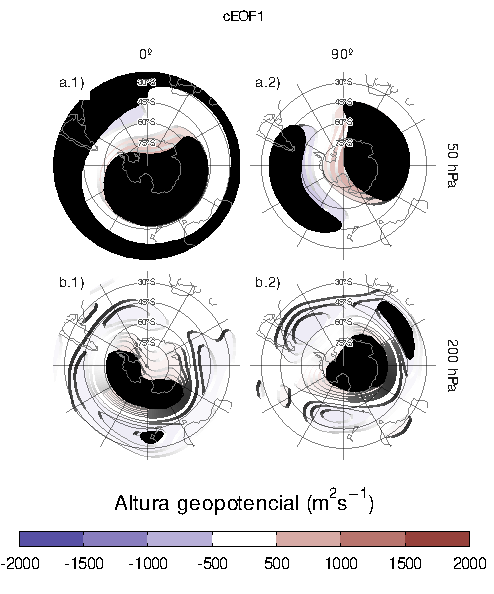
\includegraphics{thesis_files/figure-latex/eof1-regr-gh-1.pdf}
\caption{\label{fig:eof1-regr-gh}Regression of SON geopotential height anomalies (\(m^2s^{-1}\)) with the (column 1) 0º and (column 2) 90º phases of the first cEOF for the 1979 -- 2019 period at (row a) 50 hPa and (row b) 200 hPa. These coefficients come from multiple linear regression involving the 0º and 90º phases. Areas marked with dots have p-values smaller than 0.01 adjusted for False Detection Rate.}
\end{figure}
La figura \ref{fig:eof1-regr-gh} muestra mapas de regresión de anomalías de altura geopotencial SON sobre cEOF1.
A 50 hPa (Figura \ref{fig:eof1-regr-gh} fila a), el cEOF1 de 0º está asociado a un centro positivo situado sobre el Mar de Ross.
El cEOF1 de 90º está asociado a un patrón de onda 1 distintivo con un máximo sobre la costa de la Antártida Oriental.
A 200 hPa (Figura \ref(fig:eof1-regr-gh) fila b) el cEOF1 de 0º muestra un único centro de anomalías positivas que abarca la Antártida Occidental rodeado de anomalías opuestas en latitudes más bajas, con su centro desplazado ligeramente hacia el este en comparación con las anomalías de niveles superiores.
El cEOF1 de 90º muestra un patrón mucho más simétrico zonalmente que se asemeja a la fase SAM negativa (por ejemplo, \textbf{fogt2020?}).
Por lo tanto, la magnitud y la fase del cEOF1 están asociadas a la magnitud y la fase de una onda zonal principalmente en la estratosfera.


\begin{figure}
\centering
\includegraphics{thesis_files/figure-latex/eof2-regr-gh-1.pdf}
\caption{\label{fig:eof2-regr-gh}Same as Figure~\ref{fig:eof1-regr-gh} but for cEOF2.}
\end{figure}
La figura \ref{fig:eof2-regr-gh} muestra los mapas de regresión de las anomalías de altura geopotencial sobre el cEOF2.
En la troposfera (Fig. \ref{fig:eof2-regr-gh} fila a) los mapas de regresión muestran trenes de ondas similares a los identificados para los patrones cEOF2 (Fig \ref{fig:ceofs-1}).
Las anomalías de regresión asociadas con el cEOF2 de 0º están desfasadas 1/4 de longitud de onda con respecto a las asociadas con el cEOF2 de 90º.
Todos los campos tienen una onda zonal dominante 3 limitada al hemisferio occidental, sobre los océanos Pacífico y Atlántico.
El cEOF2 representa entonces un tren de ondas barotrópico equivalente muy similar al de los Patrones PSA (Mo and Paegle, 2001).
Comparando la localización de la anomalía positiva cerca de 90ºW en la columna 2 de la Figura \ref(fig:eof2-regr-gh) con las Figuras 1.a y b de Mo and Paegle (2001), el mapa de regresión 0º cEOF2 podría identificarse con PSA2, mientras que el 90º cEOF2 se asemeja a PSA1.

Estos patrones de ondas también están presentes en la estratosfera (Fig. \ref(fig:eof2-regr-gh) fila a) apoyando su naturaleza barotrópica equivalente.
Pero también está presente un monopolo sobre el polo con signo negativo asociado a los 0º cEOF2 y signo positivo asociado a los 90º cEOF2.
Este monopolo podría indicar fortalecimiento del vórtice polar asociado a valores positivos del 0º cEOF2 y debilitamiento asociado a valores negativos del 0º cEOF2.
Sin embargo, dado que estas anomalías no son estadísticamente significativas, esta característica no debe sobreinterpretarse.

\hypertarget{temperatura-y-ozono}{%
\subsubsection{Temperatura y Ozono}\label{temperatura-y-ozono}}


\begin{figure}
\centering
\includegraphics{thesis_files/figure-latex/eof1-regr-t-1.pdf}
\caption{\label{fig:eof1-regr-t}Same as Figure~\ref{fig:eof1-regr-gh} but for air temperature (K).}
\end{figure}

\begin{figure}
\centering
\includegraphics{thesis_files/figure-latex/t-vertical-1.pdf}
\caption{\label{fig:t-vertical}Regression of SON zonal anomalies averaged between 75°S and 45°S of mean air temperature (shaded, Kelvin) and ozone mixing ratio (contours, negative contours with dashed lines, labels in parts per billion by mass) with the (a) 0º and (b) 90º phase of the cEOF1 for the 1979 -- 2019 period.}
\end{figure}
También se evaluó la firma de la variabilidad de los cEOFs en la temperatura del aire.
La figura \ref{fig:eof1-regr-t} muestra los mapas de regresión de las anomalías de la temperatura del aire a 50 hPa y 200 hPa en el cEOF1.
La distribución de los coeficientes de regresión de la temperatura a 50 hPa y a 200 hPa refleja los mapas de regresión de la altura geopotencial a 50 hPa (Fig. \ref{fig:eof1-regr-gh}).
En ambos niveles, el 0º cEOF1 se asocia a un centro positivo sobre el Polo Sur con su centro desplazado ligeramente hacia 150ºE (Fig. \ref{fig:eof1-regr-t} columna 1).
Por otro lado, los mapas de regresión sobre los 90º cEOF1 muestran un patrón de onda 1 más claro con su máximo alrededor de los 60ºE.

La figura \ref{fig:t-vertical} muestra la distribución vertical de los coeficientes de regresión sobre cEOF1 a partir de anomalías zonales de la temperatura del aire y de la proporción de mezcla de ozono promediadas entre 75°S and 45°S.
Las anomalías zonales de temperatura asociadas al cEOF1 muestran un claro patrón de onda 1 tanto para la fase de 0º como para la de 90º en toda la atmósfera por encima de 250 hPa con una inversión de signo por encima de 10 hPa.
Como resultado del balance hidrostático, este es el nivel en el que la anomalía geopotencial tiene máxima amplitud (no mostrado).

Las máximas anomalías regresivas de ozono coinciden con las mínimas anomalías de temperatura por encima de 10 hPa y con las máximas anomalías de temperatura por debajo de 10 hPa (Fig. \ref{fig:t-vertical}).
Por tanto, la onda zonal 1 de ozono está correlacionada negativamente con la onda zonal 1 de temperatura en la estratosfera superior, y positivamente en la estratosfera superior.
Este cambio de fase se observa en las anomalías de ozono forzadas por ondas planetarias que alcanzan la estratosfera.
En la estratosfera superior, dominada fotoquímicamente, las temperaturas frías inhiben la destrucción de ozono, explicando el comportamiento opuesto para ambas variables, tal y como se dilucidó con modelos químicos dinámicos (\textbf{hartmann1979?}; \textbf{wirth1993?}; \textbf{smith1995?}).
Por otro lado, en la estratosfera baja dominada por la advección, las anomalías de ozono están desfasadas 1/4 de longitud de onda con el transporte horizontal y vertical, que a su vez están desfasados 1/4 de longitud de onda con las anomalías de temperatura, resultando anomalías del mismo signo para la respuesta de ambas variables (\textbf{hartmann1979?}; \textbf{wirth1993?}; \textbf{smith1995?}).


\begin{figure}
\centering
\includegraphics{thesis_files/figure-latex/o3-regr-1.pdf}
\caption{\label{fig:o3-regr}Regression of SON mean Total Column Ozone anomalies (shaded, Dobson Units) with the (a) 0º and (b) 90º phases of the cEOF1 for the 1979 -- 2019 period. On contours, the mean zonal anomaly of Total Column Ozone (negative contours in dashed lines, Dobson Units). Areas marked with dots have p-values smaller than 0.01 adjusted for False Detection Rate.}
\end{figure}


Los mapas de regresión de las anomalías del COT sobre el cEOF1 (Fig.\ref(fig:o3-regr)) muestran patrones de onda zonal 1 asociados a ambos componentes del cEOF1.
La posición climatológica del mínimo primaveral de ozono (agujero de ozono) se encuentra fuera del Polo Sur y hacia el mar de Weddell (por ejemplo, \textbf{grytsai2011?}).
Así, el campo de regresión 0º cEOF1 (Figura~\ref{fig:o3-regr}a) coincide con la posición climatológica del agujero de ozono, mientras que está desfasado 90º para el 90º cEOF1.
La correlación temporal entre las amplitudes de la onda planetaria 1 del COT y la amplitud del cEOF1 es 0.79 (CI: 0.63 -- 0.88), mientras que la correlación entre sus fases es -0.85 (CI: -0.92 -- -0.74).
En consecuencia, cEOF1 está fuertemente relacionado con la variabilidad del ozono SH.

\hypertarget{fuentes-de-variabilidad-tropicales}{%
\subsection{Fuentes de variabilidad tropicales}\label{fuentes-de-variabilidad-tropicales}}
\begin{figure*}
\includegraphics{thesis_files/figure-latex/sst-psi-2-1} \caption{Regression of SST (K, left column) and streamfunction zonal anomalies (\(m^2/s\times10^-7\), shaded) with their corresponding activity wave flux (vectors) (right column) upon cEOF2 different phases (illustrated in the lower-left arrow) for the 1979 -- 2019 period. Areas marked with dots have p-values smaller than 0.01 adjusted for FDR.}\label{fig:sst-psi-2}
\end{figure*}


También se evaluaron las conexiones entre los cEOF y las fuentes tropicales de variabilidad.
La figura \ref{fig:sst-psi-2} muestra los mapas de regresión de las anomalías de la temperatura de la superficie del mar (TSM) y de la función de corriente a 200 hPa sobre los cEOF2 normalizados.
Además de los mapas de regresión para las fases de 0º y 90º, incluimos las regresiones correspondientes para dos direcciones intermedias (correspondientes a 45º y 135º).

La cEOF2 de 90º (segunda fila) está asociada a fuertes anomalías positivas de la TSM en el Pacífico central y oriental y a anomalías negativas en una zona que atraviesa el norte de Australia, Nueva Zelanda y la Zona de Convergencia del Pacífico Sur (SPCZ) (Figura \ref@(fig:sst-psi-2).b1).
El campo de regresión de las anomalías de la TSM guarda un gran parecido con el ENOS canónicamente positivo (\textbf{bamston1997?}).
De hecho, existe una correlación significativa y muy alta (0.76 (CI: 0.6 -- 0.87)) entre el ONI y la serie temporal 90º cEOF2.
Además del patrón similar al ENOS del Pacífico, también hay anomalías positivas en el océano Índico occidental y valores negativos en el océano Índico oriental, lo que se asemeja a un DIO positivo (\textbf{saji1999?}).
De forma coherente, la correlación entre el 90º cEOF2 y el DMI es 0.62 (CI: 0.38 -- 0.78).

El 90º cEOF2 está asociado a fuertes anomalías de la función de onda que emanan de los trópicos (Figura \ref{fig:sst-psi-2}.b2), tanto del sector del Pacífico Central como del Océano Índico.
La respuesta atmosférica asociada a 90º cEOF2 es entonces consistente con el efecto combinado del ENOS y el DIO sobre los extratropicos: con anomalías de la TSM que inducen convección tropical anómala que a su vez excita ondas de Rossby que se propagan meridionalmente hacia latitudes más altas (\textbf{mo2000?}; \textbf{cai2011?}; \textbf{nuncio2015?}).

Sin embargo, el cEOF2 no está asociado a los mismos patrones de anomalía de la TSM tropical en todas sus fases Las figuras \ref{fig:sst-psi-2}.d1 y d2 muestran que la cEOF2 de 0º no está asociada a ninguna anomalía significativa de la TSM ni de la función de la corriente en los trópicos.
Como resultado, la correlación entre el 0º cEOF2 y ENSO no es significativa (0 (CI: -0.3 -- 0.31)).
Mientras tanto, las filas a y c de la Fig.\ref{fig:sst-psi-2} muestran que las fases intermedias siguen asociadas con anomalías regresivas significativas de la TSM sobre el Océano Pacífico, pero en lugares ligeramente diferentes.
La fase de 135º está asociada a anomalías de la TSM en el Pacífico central (Fig.\ref{fig:sst-psi-2}a.1), mientras que la fase de 45º está asociada a anomalías de la TSM que corresponden aproximadamente a los ``sabores'' de ENSO del Pacífico central y del Pacífico oriental, respectivamente (Fig.\ref{fig:sst-psi-2}c.1) (\textbf{kao2009?}).
Ambas fases también están asociadas a trenes de ondas que se generan en la región que rodea Australia y se propagan hacia los extratropicales, aunque menos intensos que los asociados a la fase de 90º.


\begin{figure}
\centering
\includegraphics{thesis_files/figure-latex/enso-phase-1.pdf}
\caption{\label{fig:enso-phase}SON ONI values plotted against cEOF2 phase for the 1979 -- 2019 period. Years with magnitude of cEOF2 greater (smaller) than the 50th percentile are shown as orange diamonds (green circles). Black line is the fit ONI \textasciitilde{} sin(phase) computed by weighted OLS using the magnitude of the cEOF2 as weights.}
\end{figure}
Para explorar más a fondo la relación entre el forzamiento tropical y las fases del cEOF2, la Figura \ref{fig:enso-phase} muestra el ONI trazado contra la fase del cEOF2 para cada trimestre SON entre 1979 y 2019, destacando los años en los que la magnitud del cEOF2 está por encima de la mediana.
En los años con ONI positivo (negativo), la fase cEOF2 se sitúa mayoritariamente en torno a 90º (-90º).
En las estaciones ENOS neutras, la fase cEOF2 es mucho más variable.
La línea negra de la figura \ref{fig:enso-phase} es un ajuste sinusoidal de la relación entre el ONI y la fase cEOF2.
El \(r^2\) correspondiente al ajuste es 0.57, estadísticamente significativo con valor p \textless{} 0.001, lo que indica una relación casi sinusoidal entre estas dos variables.

La correlación entre la magnitud absoluta del ONI y la amplitud del cEOF2 es 0.45 (CI: 0.17 -- 0.66).
Sin embargo, esta relación está determinada principalmente por los tres años con los eventos ENSO más intensos del periodo (2015, 1997, and 1982), que coinciden con los tres años con la magnitud CEOF2 más intensa (no se muestra).
Si se eliminan esos años, la correlación deja de ser significativa (0.04 (CI: -0.28 -- 0.35)).
Además, incluso cuando se utilizan todos los años, la correlación de Spearman -que es robusta frente a los valores atípicos- tampoco es significativa (0.2, valor p = 0.21).
Por lo tanto, aunque la localización de las anomalías tropicales de la TSM parece tener un efecto en la definición de la fase del cEOF2, la relación entre la magnitud del cEOF2 y el ONI sigue siendo incierta y podría ser sólo evidente en eventos ENSO muy fuertes, que son escasos en el registro observacional histórico.

Concluimos que el tren de ondas representado por cEOF2 puede ser tanto parte de la variabilidad interna de la atmósfera extratropical como forzado por las TSM tropicales.
En el primer caso, el tren de ondas tiene poca preferencia de fase.
Sin embargo, cuando cEOF2 es excitado por la variabilidad de la TSM tropical, tiende a permanecer bloqueado en la fase de 90º.
Esto explica la relativa sobreabundancia de años con cEOF2 cerca de la fase positiva y negativa de 90º en la figura @ref(fig:histograma de fase).

A diferencia del caso cEOF2, no hay anomalías significativas de TSM regresiva asociadas ni con la fase 0º ni con la fase 90º cEOF1 (Sup. Figura \ref{fig:sst-psi-1}).
Consistentemente, las anomalías de la función de corriente no muestran ninguna influencia tropical.
En su lugar, los cEOF1 de 0º y 90º están asociados a flujos de actividad ondulatoria que se propagan zonalmente en los extratropicales alrededor de 60ºS, excepto por un flujo hacia el ecuador desde la costa de la Antártida alrededor de 150ºE en la fase de 0º.
Esto sugiere que la variabilidad de cEOF1 está impulsada principalmente por la variabilidad interna de los extratropicales.

\hypertarget{impactos-en-superficie}{%
\subsection{Impactos en superficie}\label{impactos-en-superficie}}
\begin{figure}
\centering
\includegraphics{thesis_files/figure-latex/pp-t2m-r2-1.pdf}
\caption{\label{fig:pp-t2m-r2}Explained variance (\(r^2\) as percentage) of 2-metre temperature (row a) and precipitation (row b) anomalies by the regression upon cEOF1 (column 1) and cEOF2 (column 2).}
\end{figure}


También se exploró la influencia de la variabilidad de los cEOFs en las anomalías tanto de la temperatura del aire a 2 metros como de la precipitación en el SH.
La figura \ref{fig:pp-t2m-r2} muestra la varianza explicada de las anomalías de temperatura y precipitación a 2 metros por el modelo lineal múltiple tanto de 0º y 90º cEOF1 (columna 1), como de 0º y 90º cEOF2 (columna 2).
La varianza explicada por cEOF1 para las anomalías de precipitación y las anomalías de temperatura en la mayoría de las regiones es extremadamente baja, excepto para el extremo norte de la Península Antártica, el norte del Mar de Weddell y la costa del Mar de Ross (Fig.\ref{fig:pp-t2m-r2}a.1).

Esta falta de relación fuerte entre el cEOF1 y la TSM, la temperatura y la precipitación podría ser sorprendente teniendo en cuenta la correlación entre el cEOF1 y la SAM (Fig. \ref{fig:sam-eof-vertical} columna 1) y la correlación entre la SAM y la TSM del Pacífico Central, la temperatura al este y oeste de la Península Antártica, y con la precipitación en el oeste de Australia (\textbf{fogt2020?}).
Esto se debe principalmente a dos razones.
En primer lugar, la correlación entre cEOF1 y la SAM en la troposfera es modesta, con menos del 50\% de varianza compartida (Fig. \ref(fig:sam-eof-vertical) columna 1), por lo que no se espera que estos índices sean equivalentes.
En segundo lugar, Campitelli et al. (2022) demostró que la fuerte relación entre la SAM y las TSM del Pacífico y las anomalías de temperatura alrededor de la Península Antártica se debe principalmente a la parte asimétrica de la SAM.
Mientras tanto, el cEOF1 está significativamente correlacionado sólo con la parte simétrica de la SAM (Fig. \ref(fig:sam-eof-vertical) columna 1), que por sí misma no está significativamente correlacionada con las temperaturas superficiales en esa zona.

Por otro lado, la varianza explicada cEOF2 es superior al 50\% en algunas regiones para ambas variables (Fig.\ref{fig:pp-t2m-r2} columna 2).
Para la temperatura de 2 metros, hay valores altos en el Pacífico tropical y en la SPCZ, así como en la región que sigue un arco entre Nueva Zelanda y el Atlántico Sur, con valores más altos en el Océano Austral.
Sobre los continentes, hay valores moderados de alrededor del 30\% de varianza explicada en el sur de Australia, el sur de Sudamérica y la Península Antártica.
En cuanto a las precipitaciones, los valores son elevados en los trópicos.
En latitudes más altas, se observan valores moderados sobre el este de Australia y algunas regiones del sur de Sudamérica.

Dado que el cEOF1 tiene una señal relativamente débil en las variables de superficie exploradas aquí, sólo nos centraremos en la influencia del cEOF2.
En la \href{mailto:figura@ref}{\nolinkurl{figura@ref}}(fig:pp-temp-2) se muestran mapas de regresión de las anomalías de temperatura a 2 metros (columna 1) y precipitación (columna 2) sobre diferentes fases del cEOF2 normalizado.


\begin{figure}
\centering
\includegraphics{thesis_files/figure-latex/pp-temp-2-1.pdf}
\caption{\label{fig:pp-temp-2}Regresión de la temperatura media de 2 metros SON (K, sombreado) y la altura geopotencial de 850 hPa (m, contornos) (columna 1), y la precipitación (correlación, columna 2) sobre diferentes fases de cEOF2. Para el periodo 1979 -- 2019. Las áreas marcadas con puntos tienen valores p inferiores a 0,01 ajustados para la tasa de detección de falsos.}
\end{figure}
Las anomalías de temperatura asociadas a los 90º cEOF (Fig.~\ref{fig:pp-temp-2}.b1) muestran valores positivos en el Pacífico tropical, coherentes con las anomalías de TSM asociadas a la misma fase (Fig.~\ref{fig:sst-psi-2}.b1).
En latitudes más altas existe un patrón ondulatorio de valores positivos y negativos que coincide con los nodos de los patrones de regresión de la altura geopotencial de 850 hPa.
Esto es coherente con las anomalías de temperatura producidas por la advección meridional de temperatura por los vientos meridionales derivados del equilibrio geostrófico.
Sobre los continentes, el 90º cEOF2 (Fig.\ref(fig:pp-temp-2)b.1) se asocia con anomalías de temperatura de regresión positiva en el sur de Australia y anomalías de regresión negativa en el sur de Sudamérica y la Península Antártica, que son resultado del tren de ondas descrito anteriormente.

Las anomalías de temperatura asociadas al 0º cEOF2 (Fig.\ref(fig:pp-temp-2)d.1) son menos extensas y se limitan a latitudes medias y altas.\\

Sobre los continentes, las regresiones de las anomalías de temperatura no son significativas, excepto las anomalías positivas cerca de la Península Antártica.

Las anomalías de precipitación tropical asociadas con el 90º cEOF2 son fuertes, con anomalías positivas en el Pacífico central y el Índico occidental, y anomalías negativas en el Pacífico oriental (Fig.\ref{fig:pp-temp-2}b.2).
Este campo es consistente con el mapa de regresión de la TSM (Fig.\ref{fig:pp-temp-2}b.1) ya que las anomalías positivas de la TSM potencian la convección tropical y las anomalías negativas de la TSM la inhiben.

En los extratropicales, el 90º cEOF2 positivo está relacionado con condiciones más secas sobre el este de Australia y el océano circundante, que es una señal similar a la asociada con ENSO (\textbf{cai2011?}).
Sin embargo, el 90º cEOF2 no es la fase más correlacionada con las precipitaciones en esa zona.
La componente de la fase 135º (una intermedia entre las positivas de 90º y 180º cEOF2) está asociada con correlaciones temporales más fuertes y extensas con la precipitación sobre Australia y Nueva Zelanda.
La influencia del cEOF2 en la precipitación australiana podría estar más relacionada con los impactos directos de las anomalías de la TSM en los océanos circundantes que en el patrón de interconexión representado por el cEOF2.

Sobre Sudamérica, el 90º cEOF2 tiene correlaciones positivas con la precipitación en el sudeste de Sudamérica (SESA) y el centro de Chile, y correlaciones negativas en el este de Brasil.
Este campo de correlación coincide con la firma de precipitación primaveral de ENSO (e.g. \textbf{cai2020a?}) y también es similar a las anomalías de precipitación asociadas con el A-SAM (Campitelli et al., 2022).
Este resultado no es sorprendente teniendo en cuenta la estrecha relación del 90º cEOF2 tanto con el ONI como con el índice A-SAM, demostrada anteriormente.
Además, consolida la identificación del cEOF2 con el patrón PSA.
Semejante a la relación entre ONI y la fase de cEOF2 (Fig.\ref{fig:enso-fase}), existe una dependencia de fase de cEOF2 de las anomalías de precipitación en SESA (no mostrado).

Los coeficientes de correlación entre las anomalías de precipitación y el 0º cEOF2 (Fig.~\ref{fig:pp-temp-2}d.2) son más débiles que para 90º cEOF2.
Hay una correlación positiva residual en el Pacífico oriental ecuatorial y pequeñas correlaciones positivas, no estadísticamente significativas, sobre el este de Australia y negativas sobre Nueva Zelanda.

\hypertarget{otras-estaciones}{%
\section{Otras estaciones ??}\label{otras-estaciones}}

Definitivamente extender al resto del año.
(índice mensual).
Esto faltaría.
Hay código para hacerlo, pero falta la interpretación, que es lo importante.

Sería un análisis más modesto.

\hypertarget{estructura-simuxe9trica-y-asimuxe9trica-del-sam}{%
\chapter{Estructura simétrica y asimétrica del SAM}\label{estructura-simuxe9trica-y-asimuxe9trica-del-sam}}

\hypertarget{datos-y-muxe9todos-1}{%
\section{Datos y métodos}\label{datos-y-muxe9todos-1}}

Acá iría gran parte \href{https://github.com/eliocamp/asymsam}{del paper del SAM}. Adentrar un poco más en la relación con el cEOF2

\hypertarget{relaciuxf3n-con-otros-patrones}{%
\chapter{Relación con otros patrones}\label{relaciuxf3n-con-otros-patrones}}

Acá seguiría parte \href{https://github.com/eliocamp/shceof}{del paper de cEOF}.

\hypertarget{datos-y-muxe9todos-2}{%
\section{Datos y métodos}\label{datos-y-muxe9todos-2}}

\hypertarget{sam}{%
\section{SAM}\label{sam}}


\begin{figure}
\centering
\includegraphics{thesis_files/figure-latex/sam-eof-vertical-1.pdf}
\caption{\label{fig:sam-eof-vertical}Coefficient of determination (\(r^2\)) between each component of cEOFs and the SAM, Asymmetric SAM (A-SAM) and Symmetric SAM (S-SAM) indices computed at each level for the 1979 -- 2019 period. Thick lines represent estimates with p-value \textless{} 0.01 corrected for False Detection Rate (\textbf{benjamini1995?}).}
\end{figure}
Ahora exploramos la relación entre SAM y los cEOFs motivados por el parecido entre los mapas de regresión de los cEOFs y los patrones de SAM mostrados en la Sección \ref{regresiones}.
Calculamos el coeficiente de determinación entre las series temporales de los cEOFs y los tres índices SAM (SAM, A-SAM y S-SAM) definidos por Campitelli et al. (2022) en cada nivel vertical (Fig.~\ref{fig:sam-eof-vertical}).
El índice SAM está correlacionado de forma estadísticamente significativa con el 0º cEOF1 en todos los niveles, y con los 90º cEOF1 y 90º cEOF2 en la troposfera.
Por otro lado, las correlaciones entre SAM y el 0º cEOF2 no son significativas.

La relación entre la SAM y el cEOF1 en la troposfera se explica en su totalidad por el componente zonalmente simétrico de la SAM, como muestran la alta correlación con la S-SAM por debajo de 100 hPa y las correlaciones bajas y estadísticamente no significativas entre la A-SAM y el 0º o el 90º cEOF1.
En la estratosfera, la CEOF1 de 0º está correlacionada tanto con la A-SAM como con la S-SAM, mientras que la CEOF1 de 90º está altamente correlacionada sólo con la A-SAM.
Estas correlaciones son consistentes con los mapas de regresión de la altura geopotencial en la Figura \ref{fig:eof1-regr-gh} y su comparación con los obtenidos para SAM, A-SAM y S-SAM por Campitelli et al. (2022).

En el caso de 90º cEOF2, su correlación con la SAM para la troposfera está asociada a la variabilidad asimétrica de la SAM.
De hecho, el 90º cEOF2 comparte hasta varianza con el A-SAM y sólo como máximo con el S-SAM (Figura \ref{fig:sam-eof-vertical}.
b2).
Esta altísima correlación entre A-SAM y 90º cEOF2 sugiere que los modos obtenidos en este trabajo son capaces de caracterizar la componente zonalmente asimétrica de la SAM descrita previamente por Campitelli et al. (2022).

\hypertarget{psa}{%
\section{PSA}\label{psa}}


\begin{table}

\caption{\label{tab:psa-eof2}Correlation coefficients (r) between cEOF2 components and the PSA1 and PSA2 modes computed as Mo and Paegle (2001) for the 1979 -- 2019 period. 95\% confidence intervals in parenthesis. p-values lower than 0.01 in bold.}
\centering
\begin{tabular}[t]{l>{}l>{}l}
\toprule
\multicolumn{1}{c}{} & \multicolumn{2}{c}{cEOF2} \\
\cmidrule(l{3pt}r{3pt}){2-3}
PC & Real & Imaginario\\
\midrule
PSA1 & 0.26 (CI: -0.04 -- 0.53) & \textbf{0.82 (CI: 0.69 -- 0.9)}\\
PSA2 & \textbf{-0.79 (CI: -0.88 -- -0.63)} & 0.02 (CI: -0.29 -- 0.32)\\
\bottomrule
\end{tabular}
\end{table}
Dada la similitud entre las estructuras asociadas al cEOF2 (Fig. \ref{fig:eof2-regr-gh}) y los patrones de PSA documentados, estudiamos la relación entre ellos.
La tabla \ref{tab:psa-eof2} muestra las correlaciones entre los dos índices PSA y las series temporales para las fases 0º y 90º de CEOF2.
Como anticipaba visualmente la figura \ref{fig:eof2-regr-gh}, existe una gran correlación positiva entre PSA1 y 90º cEOF2, y entre PSA2 y 0º cEOF2.
Por otro lado, no existe una relación significativa entre PSA1 y 0º cEOF2, y entre PSA2 y 90º cEOF2.
En consecuencia, cEOF2 representa bien tanto la estructura espacial como la evolución temporal de los modos PSA, por lo que es posible establecer una asociación entre sus dos fases y los dos modos PSA.
Es decir, la elección de fase para cEOF2 que maximiza la relación entre ENSO y 90º cEOF2, también maximiza la asociación entre los componentes de cEOF2 y los modos PSA (no mostrado).


\begin{figure}
\centering
\includegraphics{thesis_files/figure-latex/phase-histogram-1.pdf}
\caption{\label{fig:phase-histogram}Histograma de distribución de fase de cEOF2 para el periodo 1979 -- 2019. Los intervalos están centrados en 90º, 0º, -90º, -180º con un ancho de intervalo de 90º. Las pequeñas líneas verticales cerca del eje horizontal marcan las observaciones.}
\end{figure}
La figura \ref{fig:histograma-fase} muestra un histograma que cuenta el número de estaciones SON en las que la fase cEOF2 estaba cerca de cada una de las cuatro fases particulares (positiva/negativa de las fases 0º y 90º), con las observaciones para cada estación marcadas como alfombras en el eje horizontal.
En 62\% de las estaciones cEOF2 tiene una fase similar a la fase negativa o positiva de 90º, haciendo que la fase de 90º sea la fase más común.
Esta es también la fase más correlacionada con ENSO según la definición de la fase de 0º descrita en la Sección @ref(métodos).

Por lo tanto, en virtud de ser la fase más común, la cEOF2 de 90º explica más varianza que la cEOF2 de 0º.
Por lo tanto, el análisis EOF convencional tenderá a separarlos de forma relativamente limpia, con el EOF que representa el 90º cEOF2 siempre por delante del que representa el 0º cEOF2.
Esta preferencia de fase está de acuerdo con (\textbf{irving2016?}), que encontró una distribución bimodal a la variabilidad tipo PSA (compare nuestra Figura \ref{fig:histograma-fase} con su Figura 6).

\hypertarget{enso}{%
\section{ENSO}\label{enso}}

\hypertarget{anuxe1lisis-de-estos-modos-en-los-modelos-de-cmip6}{%
\chapter{Análisis de estos modos en los modelos de CMIP6}\label{anuxe1lisis-de-estos-modos-en-los-modelos-de-cmip6}}

Acá iría el \href{https://htmlpreview.github.io/?https://github.com/eliocamp/onda3/blob/master/35-cEOF-CMIP6-superensemble-SON.html}{análisis de los cEOF en CMIP6} que ya hice. Está analizado bastante de primavera, faltaría el resto del año.

\hypertarget{datos-y-muxe9todos-3}{%
\section{Datos y métodos}\label{datos-y-muxe9todos-3}}

\hypertarget{primavera-1}{%
\section{Primavera}\label{primavera-1}}

\hypertarget{comparaciuxf3n-con-los-modos-observados}{%
\subsection{Comparación con los modos observados}\label{comparaciuxf3n-con-los-modos-observados}}

\hypertarget{tendencias}{%
\subsection{Tendencias}\label{tendencias}}

\hypertarget{otras-estaciones-1}{%
\section{Otras estaciones ??}\label{otras-estaciones-1}}

\backmatter

\hypertarget{referencias}{%
\chapter*{Referencias}\label{referencias}}
\addcontentsline{toc}{chapter}{Referencias}

\markboth{Referencias}{Referencias}

\noindent

\setlength{\parindent}{-0.20in}

\hypertarget{refs}{}
\begin{CSLReferences}{1}{0}
\leavevmode\vadjust pre{\hypertarget{ref-campitelli2022}{}}%
Campitelli, E., Díaz, L.B., and Vera, C., 2022. \href{https://doi.org/10.1007/s00382-021-05896-5}{Assessment of zonally symmetric and asymmetric components of the {Southern Annular Mode} using a novel approach}. Climate Dynamics, 58, 1, 161--178.

\leavevmode\vadjust pre{\hypertarget{ref-mo2001}{}}%
Mo, K.C., and Paegle, J.N., 2001. \href{https://doi.org/10.1002/joc.685}{The {Pacific}\textendash{{South American}} modes and their downstream effects}. International Journal of Climatology, 21, 10, 1211--1229.

\end{CSLReferences}

% Index?

\end{document}
